\section{Results}
\label{sec:results}

\subsection{Model Evaluation and Validation}
\label{subsec:eval}
There are two different scores to be considered as result, the score given by the training and test data, which performed only over known data, and the score resulted by future predictions. These scores will be defined
as \textbf{Test Score} and \textbf{Prediction Score}.\\
\\
About the \textbf{Test Score:}\\
After considering the aspects explained on subsections \ref{subsec:Exploratory_visu} and \ref{subsec:implementation}, the main model developed to perform the predictions use the \textit{Support Machine Regressor} algorithm.
Simulating the results of several companies, the $R^2 score$ reached for everyone was higher than 0.9.
All the results was achieved using the kernel \textit{RBF} with \textit{Pipeline} in order to obtain the best possible parameters.
However, it is necessary to display the results in a understandable and efficient visualization. This objective was reached using \textit{google's chart API} for HTML. 
This solution allows the user to interact with the graph in an easier form, understanding better what is being predicted.\\
\\
This model is robust enough for this problem and performs with a high accuracy. Small changes are being rightly predict, but, as explained in the section \ref{sec:definition}, the scope of this project is not to predict when a drastic fall
(or rise) of stock shares will occur. Therefore, in order to understand better the stock prices of some companies and to predict if it might be a good option to buy or sell shares in a short term, the algorithm implemented is robust. 
The graphs generated by this algorithm will be displayed in the next subsection.\\
\\
Until the final model was no decided, some others model were stressed in order to obtain great results. 
These models are available, when using the \textit{app} developed for this project, to be selected and executed. 
An algorithm of \textit{deep learning} is implemented, however, it is not optimized to work with different data, which makes it unstable to be used.\\
\\
About the \textbf{Prediction Score:}\\
Using the learner acquired by last simulation, was separeted the last 10 days of the dataset, to visualize how the predictor would perform. The score achieved was of 0.2229. The Figure \ref{fig:pred_10} 
compares the data of these 10 days, the smooth curve used in the predictor and the predictor.
\begin{figure}[H]
\centering
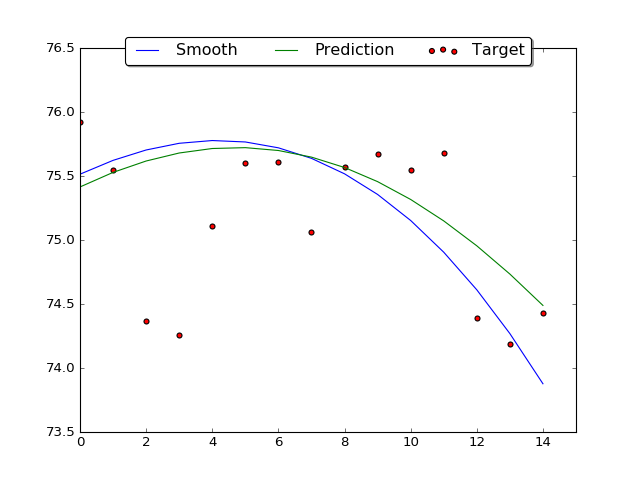
\includegraphics[width=0.6\textwidth]{figures/pred_10.png}
\caption{NVS: 10 days of prediction}
\label{fig:pred_10}
\end{figure}
\ \\


\subsection{Justification}
As explained in subsection \ref{subsec:eval}, there are two scores considered. Firstly it will be showed this results, and the predictions performed with them, then a comparison between the bechmark and the 
wanted score.\\
\\
\textbf{Test Score}\\
Results achieved for the company \textit{NVS - Norvatis AG Common Stock}.
The Figure \ref{fig:predict_svr} presents the results in two parts: 
\begin{itemize}
	\item Text: It contains three informations: The specific algorithm used, the  score reached with the test data and the parameters used with the model.\\
	\item Graph: The historical data and the predict data for the \textit{Adjustment Closing Prices}.\\
\end{itemize}

\begin{figure}[H]
\centering
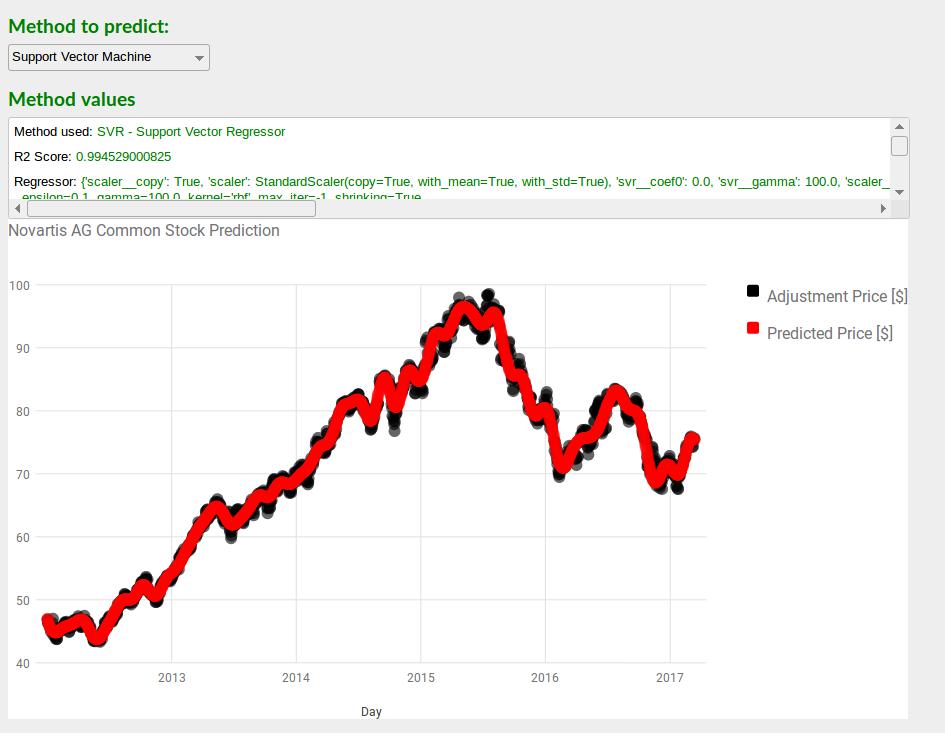
\includegraphics[width=0.6\textwidth]{figures/predict_svr.png}
\caption{NVS: Prediction Results and Historical Data}
\label{fig:predict_svr}
\end{figure}
\ \\

The score reached in this simulation was $0.9945$, which means that $99,45\%$ of the test subset data was predicted correctly. 
This score is higher than the wished benchmark in the beginning of this project. The graph, comparing historical data with all the data predicted by the model, 
is displayed to the user in order to clarify what this score means. After the model is trained, it is possible to predict the next days of the stock prices. 
The Figure \label{fig:predict_45days} displays the results. Since the Stock Market does not open every day, the sequence of the 45 days predicted in this image is wrongly named. 
It should be considered on working days. 

\begin{figure}[H]
\centering
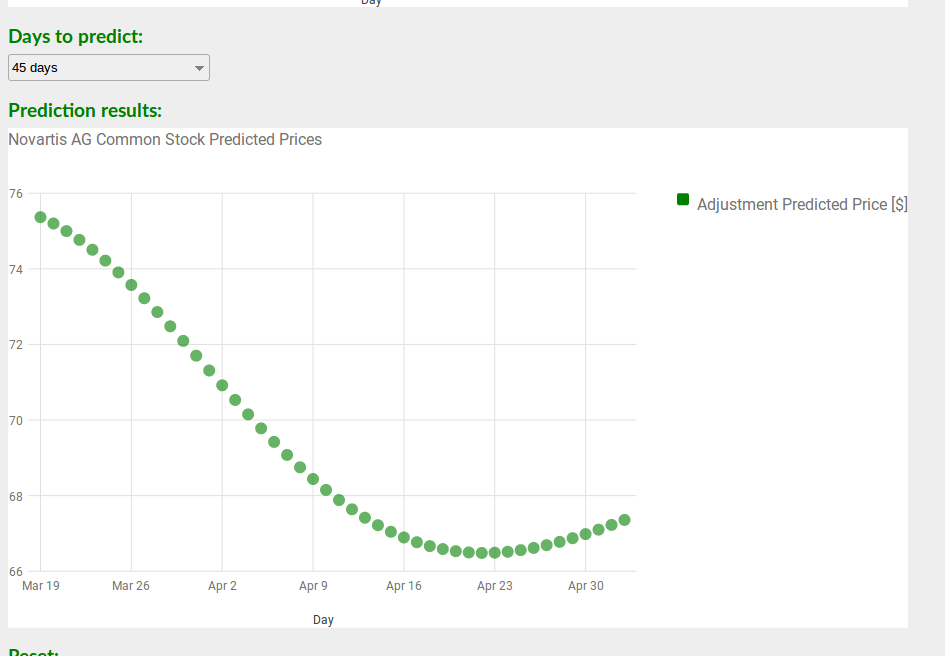
\includegraphics[width=0.6\textwidth]{figures/predict_45days.png}
\caption{NVS: Prediction Results for 45 days}
\label{fig:predict_45days}
\end{figure}
\ \\

\textbf{Prediction Score}\\
After the score achieved with the simulation of the last 10 days, presented in subsection \ref{subse:eval}, it is clear that this model is not efficient. Still, this is a better
solution than a random guess. As demonstraed in Figure \ref{fig:pred_10}, the result tends to follow the prices, however with time it gets higer errors. Therefore, this model
could work for a short term prediction, as one or two days, just to understand the value of the shares.
The next section will consider the improvements that can be done for this project in order to achieve better results, 
and explain how they can be implemented. \\